\documentclass[main]{subfiles}
\begin{document}

%@@@@@@@@@@@@@@@@@@@@@@@@@@@@@@
%\noindent
%\textbf{Topics: Digital logic, Linear Threshold Unit/Gates, Introduction to Perceptron Learning Algorithm - 21.11.2019} \\
%Lecturer: Dr. Matthew Cook \\
%Author: Vanessa Leite \{vanessa at ini.uzh.ch\}

\section{Introduction to Perceptron Learning Algorithm}

We don't learn how the brain works by studying neurons, the same way that just by studying transistors we do not know how a computer works.
We know the brain does processing but we don't know how it works.
The bottleneck to understand brain is probably that we do not have the right abstractions to understand it.

McCulloch and Pitts developed a computational model of a biological neuron in 1943.
The McCulloch-Pitts neural model is also known as linear threshold unit/gate. It is a neuron with a set of inputs and one output.

\subsection{McCulloch-Pitts neurons vs biological neurons}
\textbf{similarities:}
\begin{itemize}[noitemsep,nolistsep]
	\item Both can be active or inactive.
	\item The input/output is directed.
	\item The activation of a neuron is dependent on a weighted function of other neurons.
\end{itemize}
\textbf{differences:}
\begin{itemize}[noitemsep,nolistsep]
	\item Real neurons exist in continuous time, whereas McCulloch-Pitts neurons operate in discrete time.
	\item Real neurons have degrees of activation, not just on/off.
	\item The activation as a function of the inputs of real neuron is typically not linear or threshold linear.
\end{itemize}

\subsection{(Basic) Digital Logic}

Gates are processing units.

\begin{figure}[H]
	\centering
	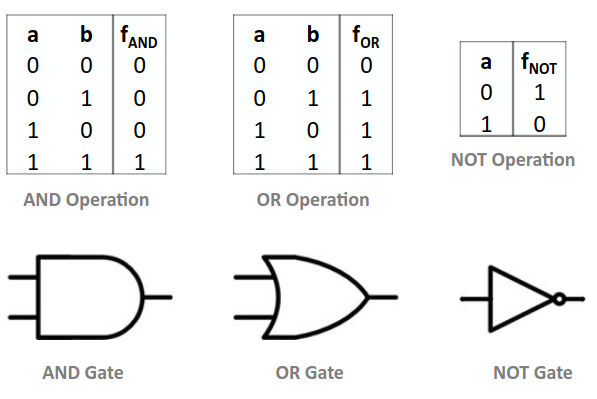
\includegraphics[width=0.5\textwidth]{basic-gates.png}
\end{figure}

Circuits are a combination of gates.

\begin{figure}[H]
	\centering
	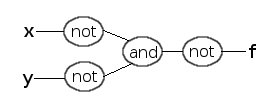
\includegraphics[width=0.4\textwidth]{circuit.png}
	\caption{A basic circuit implementing an OR gate.}
	\label{fig:circuit-gates}
\end{figure}

The circuit in Figure~\ref{fig:circuit-gates} produces the same output as an OR gate.
With NOT and AND gates we can build an OR gate, but with AND and OR we can't build a NOT gate.

\paragraph{XOR gates = exclusive OR}
They are exclusive in the case of two inputs.
For more than two, XOR counts the number of "active" ($1$'s) inputs and returns $0$ for even and $1$ for odd.

\begin{figure}[H]
	\centering
	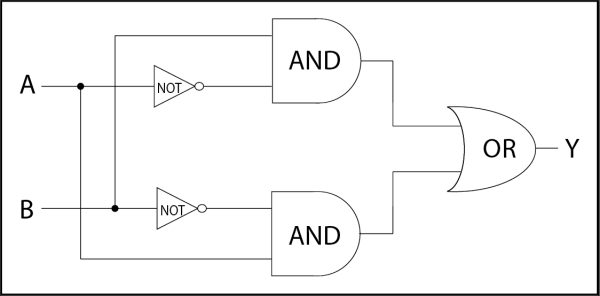
\includegraphics[width=0.5\textwidth]{gatexor.png}
	\caption{XOR gate built out other gates. Image from https://blog.digilentinc.com/building-logic-gates-with-transistors/}
	\label{fig:xor-gates}
\end{figure}

A table with $N$ inputs has $2^N$ rows.

\paragraph{Other gates}

\begin{tabular}{|c|c|c|c|c|c|c|c|c|}
	\hline
	\multicolumn{2}{|c|}{Input} &
	\multicolumn{7}{|c|}{Output}\\\hline
	A & B & AND & OR & NOT & XOR & NAND & NOR & XNOR\\\hline
	  &   & \scalebox{0.4}{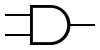
\includegraphics{100px-AND_ANSI.png}} & \scalebox{0.4}{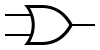
\includegraphics{100px-OR_ANSI.png}} &\scalebox{0.4}{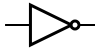
\includegraphics{100px-NOT_ANSI.png}} &\scalebox{0.4}{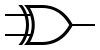
\includegraphics{100px-XOR_ANSI.png}} &\scalebox{0.4}{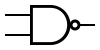
\includegraphics{100px-NAND_ANSI.png}} &\scalebox{0.4}{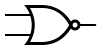
\includegraphics{100px-NOR_ANSI.png}} &\scalebox{0.4}{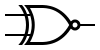
\includegraphics{100px-XNOR_ANSI.png}}\\\hline
	0 & 0 & 0 & 0 & 1 & 0 & 1 & 1 & 1\\\hline
	0 & 1 & 0 & 1 & 1 & 1 & 1 & 0 & 0\\\hline
	1 & 0 & 0 & 1 & 0 & 1 & 1 & 0 & 0\\\hline
	1 & 1 & 1 & 1 & 0 & 0 & 0 & 0 & 1\\\hline
\end{tabular}

\subsection{Linear Threshold (LT) Unit/Gates (Perceptron)}

\begin{figure}[H]
	\centering
	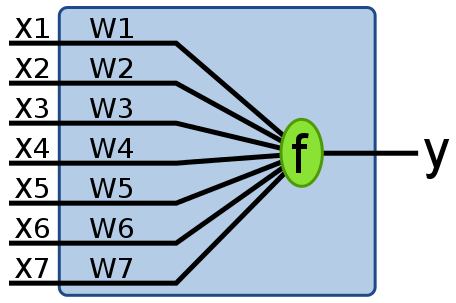
\includegraphics[width=0.3\textwidth]{perceptron.png}
\end{figure}

This model represents a neuron with inputs $x$ and one output $y$.
Weights $w$ determine the influence of the inputs.
$f$ is a function determining the output: if the influence of all the inputs combined cross a threshold, then the neuron become active.
Active state: $\sum_i(w_i\cdot x_i) \geq \theta$.
Otherwise, the neuron is inactive.

We add a bias input as $-\theta$ so that $w_0+\sum_i(w_i\cdot x_i)\geq0$ activates the neuron.
As a digital abstraction, we consider that the activity of a neuron can be described as $0$ or $1$. Where $0$ is inactive and $1$ is active.

Neurons can learn by adjusting their weights, they can have thousand of inputs.
For a desired behavior there are many possible weight vectors that can work (if any can work). 
This model can create AND/OR/NOT-Gates.

\subsubsection{Threshold function}

\begin{figure}[H]
	\centering
	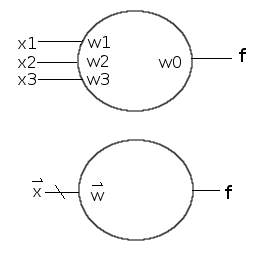
\includegraphics[width=0.2\textwidth]{simplified-LT.png}
	\caption{Same unit in two representations}
	\label{fig:simplified-LT}
\end{figure}

Both units in Figure~\ref{fig:simplified-LT} are the same.
The one in the bottom is a simplified version, where the inputs $x$ and the weights $w$ are represented as vectors.
The bias term is added to the weight vector and a new input $x_0$ is added with a fixed value of $1$.\\
$f(x_1, x_2, x_3) = \theta(w_1 \times x_1 + w_2 \times x_2 + w_3 \times x_3 + w_0)$\\
$f(\vec{x}) = \theta(\vec{w} \times \vec{x} + w_0)$\\

\[
  \theta(x)=
  \begin{cases}
     0 \text{, if } x < 0\\
     1 \text{, if } x \geq 0\\
  \end{cases}
\]

\subsubsection{XOR impossibility with LT/Perceptrons}
To compute XOR with LT, it is required that:

\begin{itemize}[noitemsep,nolistsep]
	\item $w_0 < 0$
	\item $x_2 \times w_2 + w_0 \geq 0$
	\item $x_1 \times w_1 + w_0 \geq 0$
	\item $x_1 \times w_1 + x_2 \times w_2 + w_0 < 0$.
\end{itemize}

This causes a contradiction because $x_1 \times w_1 + x_2 \times w_2 + 2 \times w_0 < 0$ and $x_1 \times w_1 + x_2 \times w_2 + 2 \times w_0 \geq 0$ when adding up the constraints.

XOR is not a linear combination of the inputs.
And the perceptron/LT uses a line to separate classes, i.e., all the points in the same side of the line will have the same output.
Although these units can't model the XOR, they are still powerful.
You can't calculate it with a single unit, but with a combination of them, it is possible.
The same way, one cannot compute the XOR function using one single OR, NOT or AND gate.
In fact, we need three gates\footnote{when couting gates, we do not count NOT gates} to compute the XOR function, see Figure~\ref{fig:xor-gates}.

In the end, these model of neuron units are more efficient than digital logic gates, however, these new analog units run into precision problems.
For implementing the XOR function, McCulloch and Pitts units allow exponentially smaller circuits.

\subsection{Perceptron Learning Algorithm}

\begin{table}[H]
\centering
\begin{tabular}{cc|c}
x1 & x2 & f \\ 
\hline
0  & 0  & 1 \\
0  & 1  & 0 \\
1  & 0  & 1 \\
1  & 1  & 1 \\ 
\end{tabular}
\caption{Two inputs $x1$ and $x2$ resulting in $f$}
\label{tab:simple_function}
\end{table}

\paragraph{Supervised error-correcting rules}
We start with an initial guess of weights, compare the output in response to the input with the desired output and change the weights to improve the performance. \\

Consider the mapping on the Table~\ref{tab:simple_function}.
Can we set $w_0, w_1, w_2$ (bias term, and the weights of each input) so that this unit computes the $f$ from the table?
Learning happens by changing synaptic weights.
How can we change the synaptic weights of a unit to make it behave as desired?

Let's start with random weights, let's say all zero.
With this weights, doesn't matter the values of $x_1$ and $x_2$, the result will always be 1.
And for the second case ($x_1 = 0, x_2 = 1, f = 0$) we produce a wrong output.
So, we reduce $w_0$ and $w_2$ because they contribute to the sum ($0 \times w_1 + 1 \times w_2 + w_0$).
We reduce the weights if the sum should go down and we increase the weights if the sum should go up. We iterate this step until convergence.

We can consider the bias as a weight with input value always one ($x_0 = 1$), thus, we can write:

\[ f(\vec{x}) = \theta(\vec{w} \times \vec{x} + w_0) = \theta(\vec{w} \times \vec{x}) \]

\paragraph{Recall} $\vec{w} \times \vec{x} = |\vec{w}| \times |\vec{x}| \times \cos \alpha$.
So, if $\alpha < 90\deg$, $\vec{w} \times \vec{x}$ is greather than zero and if $\alpha > 90\deg$, $\vec{w} \times \vec{x} < 0$.
This way, we compute a similarity between the weight vector and the input vector. \\

\subsubsection{Convergence}
These single units can separate two classes if they are linearly separable (i.e., if a solution exists). The Perceptron Learning Algortithm must converge, i.e., it will update the weights a finite number of times.

\paragraph{Proof 1}
Suppose there is a solution $\vec{w}^*$, i.e., the data is linearly separable.
The weights of the perceptron units can be seen as the components of a normal vector to the hyperplane that separates the classes ($1$ and $0$).
In  fact, the  length of the normal vector doesnt matter, we are looking for its direction.
Pick any solution $\vec{w}$, for instance, starting with all weights as zero, if this solution already satisfies our conditions, we are done.
Otherwise, we pick an arbitrary missclassified point and update $\vec{w}$.
Each step makes progress in the $\vec{w}^*$ direction, because additions to $\vec{w}$ are always $\leq 90\deg$.
The magnitude of $\vec{w}^* \times \vec{w}$ increases linearly.
Since $\vec{w}^*$ doesn't change, there is a maximum growth from $\vec{w}$ to achieve the solution.
By contradiction in the limit of infinite steps, we can say that the algorithm converges, i.e., if there is a solution and it takes infinite steps to achieve it, this is a contradiction.

\paragraph{Proof 2}
In homogeneous coordinates $\mathcal{\hat{X}}^{\prime}_{n} \equiv \{ \hat{x}^{\prime}_{i} = l_i \hat{x}_i | (x_i, l_i) \in \mathcal{\hat{X}}_{n} \}$.
\begin{itemize}
\item $\hat{w}^{*}$ (solution) $\in \mathbb{R}^{n+1}$ is the homogeneous weight vector: $\hat{w}^T \hat{x}^{\prime}_i > 0, \forall i = 1, \dots, n$.
\item $hat{w}(k) \in \mathbb{R}^{n+1}$ is the homogeneous weight vector of the $k-$th update.
\item $\hat{x}^{\prime}(k) \in \mathcal{\hat{X}}^{\prime}_n$ is the normalized homogeneous feature vector that triggered the update.
\end{itemize}
Then, $\hat{w}(1) = \hat{w}(0) + \eta \hat{x}^{\prime}(1)$, $\hat{w}(2) = \hat{w}(1) + \eta \hat{x}^{\prime}(2)$, $\hat{w}(3) = \hat{w}(2) + \eta \hat{x}^{\prime}(3)$, $\dots$, $\hat{w}(k) = \hat{w}(k-1) + \eta \hat{x}^{\prime}(k)$.
Can we find two constants $A$ and $B$ such that:
\begin{equation}
Ak^2 \leq || \hat{w}(k) - \hat{w}(0) || \leq Bk
\label{eq:convergence}
\end{equation}
?

\begin{figure}[H]
	\centering
	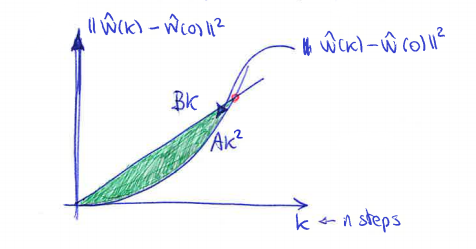
\includegraphics[width=0.7\textwidth]{pla_convergence_proof.png}
	\caption{The space of searching for the solution has an upper and a lower bound.}
	\label{fig:simplified-LT}
\end{figure}
If~\ref{eq:convergence} holds then the growth of $\hat{w}(k)$ is limited.
As $k$ increases, $Bk$ will be smaller then $Ak^2$.
For~\ref{eq:convergence} to hold, $|| \hat{w}(k) - \hat{w}(0) ||$ cannot increase after $k = \frac{B}{A}$ updates.

We show that the vector that is the difference between the original vector and the $k-$th one is limited: the algorithm must converge.

\textbf{Lower bound $A$}:\\
\indent \indent $\hat{w}(k) = \hat{w}(0) + \eta (\hat{x}^{\prime}(1) + \hat{x}^{\prime}(2) + \dots + \hat{x}^{\prime}(k))$\\
\indent \indent $\hat{w}^{*T} (\hat{w}(k) - \hat{w}(0)) = \hat{w}^{*T} \eta (\hat{x}^{\prime}(1) + \hat{x}^{\prime}(2) + \dots + \hat{x}^{\prime}(k))$ \\
\indent \indent Given $a = \min_{\hat{x} \in \hat{\mathcal{X}}^{\prime}_{m}} \hat{w}^{*T} \hat{x}^{\prime} > 0$ then $\hat{w}^{*T}(\hat{w}(k) - \hat{w}(0)) \geq \underbrace{\eta a k}_{\text{summing $k$ times the minimum term}} > 0$\\
\indent \indent From the Cauchy-Schwartz: $\| a \|^2 \| b \| ^2 > |a^T b |^2$\\
\indent \indent $\|\hat{w}^{*T}\|^2 \|\hat{w}(k) - \hat{w}(0) \|^2 > | \hat{w}^{*T} (\hat{w}(k) - \hat{w}(0)|^2 \geq (\eta a k )^2$ \\
\indent \indent $\rightarrow \| \hat{w}(k) - \hat{w}(0)\|^2 \geq \underbrace{\left( \frac{\eta a}{\| \hat{w}^* \|} \right)^2}_{A} k^2$.\\

\textbf{Upper bound $B$}:\\
\indent \indent $\hat{w}(1) - \hat{w}(0) = \eta \hat{x}^{\prime}(1)$\\
\indent \indent $\hat{w}(k) - \hat{w}(0) = (\hat{w}(k-1) - \hat{w}(0)) + \eta \hat{x}^{\prime}(k)$\\
\indent \indent $\| \hat{w}(1) - \hat{w}(0) \| ^2 = \eta \|\hat{x}^{\prime}(1) \|^2$\\
\indent \indent $\| \hat{w}(k) - \hat{w}(0) \|^2 = \| \hat{w}(k-1) - \hat{w}(0)\|^2 + 2 \eta (\| \hat{w}(k-1) - \hat{w}(0)\|^2)^T \hat{x}^{\prime}(k) + \|\hat{x}^{\prime}(k)\|^2 \eta^2$\\
\indent \indent Since $\hat{x}^{\prime}(1)$ triggers the first update, then $\hat{w}(0)^{T} \hat{x}^{\prime}(1) <0 \rightarrow \hat{w}(j-1)^T \hat{x}^{\prime}(j) < 0$ $\forall j = 1, \dots, k$\\
\indent \indent Summing up the above: $\| \hat{w}(k) - \hat{w}(0) \|^2 \leq \| \hat{w}(k-1) - \hat{w}(0)\|^2 + B^2$\\
\indent \indent By induction: $\| \hat{w}(k) - \hat{w}(0) \|^2 \leq k B^2$\\

\textbf{Combining the bounds:}\\
\indent \indent $k^2 A \| \leq \| \hat{w}(k) - \hat{w}(0) \|^2 \leq k B^2$\\
\indent \indent from which follows that $k \leq \frac{B^2}{A}$. So, the number of errors the PLA makes is finite.

\paragraph{Algorithm}
\begin{itemize}[noitemsep,nolistsep]
	\item Choose random initial weights.
	\item Calculate output for given input.
	\item If the output is not the expected value, then $e=d-c$, where $d$ is the desired output and $c$ the current output.
	\item Change the weight of inputs and bias by $\Delta w_i=e\cdot\alpha\cdot x_i$. For the bias, always use $x=1$.
\end{itemize}

\subsection{Converting real weights to integer}
Any unit can be converted into one with integer weights.

\begin{figure}[H]
	\centering
	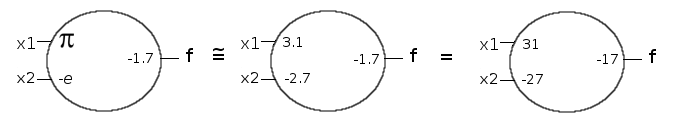
\includegraphics[width=0.8\textwidth]{converting-units-integer.png}
	\caption{Converting real weights to integer}
	\label{fig:converting}
\end{figure}

Figure~\ref{fig:converting} shows the approach to convert real weights to integer. The approximation (images left and center) can be problematic if $x$ in $\theta(x)$ is equal to zero (in the real setup), because it can be shifted in uthe approximation.
In the second step (images center and right) there is no problem. By multiplying the weights by a factor of 10, we do not change the value of $x$ in $\theta(x)$.

One way to solve the above problem (approximation) is to shift the bias term a bit.

\begin{enumerate}
\item Find the largest possible negative sum (closest to zero)
\item Adjust bias (increase) if necessary, so no sum is zero
\item Replace weights with rational approximations more precise than sum closest to zero
\item Scale up weights to be integers
\end{enumerate}

In the first two steps, we avoid have a sum of zero. On the last two, we transform the weights to integer.

So far, the difference of this unit and a real neuron is that neurons can adjust their own weight (learning) and these units are behaving as gates.

\end{document}
